\chapter{PENGUJIAN DAN ANALISIS}
\label{chap:pengujiananalisis}

% Ubah bagian-bagian berikut dengan isi dari pengujian dan analisis

Pada bab ini akan dipaparkan mengenai beberapa hasil pengujian sesuai dengan telah dijelaskan pada metodologi. Hasil pengujian ini dilakukan guna untuk mendapatkan hasil klasifikasi dan deteksi yang optimal. Pelaksanaan metodologi serta hasil pengujian yang akan dipaparkan dalam bab ini diharapkan dapat memberikan pemahaman mengenai hasil dan pembahasan sehingga dapat ditarik kesimpulan dari Tugas Akhir yang telah dilaksanakan.


\section{Pengujian Klasifikasi Menggunakan CNN 2-Dimensi}
\label{sec:PengujianCNN2D}
Proses klasifikasi menggunakan CNN 2-Dimensi dilakukan sebanyak tiga kali percobaan. Pada setiap percobaan, dilakukan training dengan pengaturan CNN 2-Dimensi yang sama kecuali dalam satu hal. Setiap percobaan dilakukan dengan pembagian jumlah data berbeda-beda untuk training, valiation, dan testing. Dari hasil tersebut akan dilakukan variasi struktur CNN 2-Dimensi dengan pembagian dataset yang memiliki hasil yang baik. Hasil klasifikasi menggunakan CNN 2-Dimensi akan dibandingkan dengan hasil klasifikasi menggunakan Roboflow dan CNN 2-Dimensi pada percobaan yang lain. Pada pengujian CNN 2-Dimensi ini nantinya akan digunakan gambar yang sama dalam masing-masing eksperimen.

\subsection{Percobaan Pertama}
Pada percobaan pertama, data yang digunakan untuk training, validation, dan testing masing-masing sebanyak 70\%, 20\%, dan 10\%. Hasil klasifikasi menggunakan CNN 2-Dimensi pada percobaan pertama mendapatkan tingkat akurasi training sebesar 0.9918 dengan training loss sebesar 0.0235. Sementara itu, didapatkan tingkat akurasi validasi sebesar 1.0 dengan valiation loss sebesar 4.6915e-05. Berikut ini adalah grafik model accuracy dan model loss pada percobaan pertama yang dapat dilihat pada Gambar \ref{fig:trainres1}.

\begin{figure} [H] \centering
    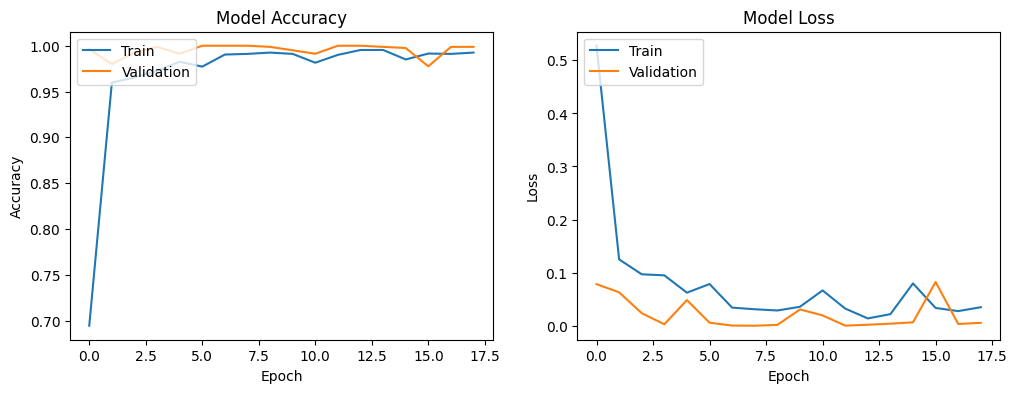
\includegraphics[scale=0.5]{gambar/bab4/trainres1.png}
    \caption{Grafik Akurasi dan Loss Model Percobaan Pertama}
    \label{fig:trainres1}
\end{figure}

Selain itu, didapatkan pula hasil confusion matrix dari data training, validation, dan testing pada percobaan pertama yang masing-masing dapat dilihat pada Gambar \ref{fig:tvcon1} dan \ref{fig:testcon1}. Dari hasil tersebut, dapat dilihat bahwa hasil klasifikasi menggunakan CNN 2-Dimensi pada percobaan pertama memiliki tingkat akurasi yang cukup tinggi. Hal ini didukung dengan nilai f1 score pada data training sebesar 0.98926264, validation sebesar 1.0, dan testing sebesar 0.99750614. Inference time yang didapatkan pada percobaan pertama untuk data training sebanyak 2804 data adalah 79 detik (283ms/step), untuk data validation sebanyak 800 data adalah 9 detik (117ms/step), dan untuk data testing sebanyak 400 data adalah 164 detik (4s/step).

\begin{figure} [H] \centering
    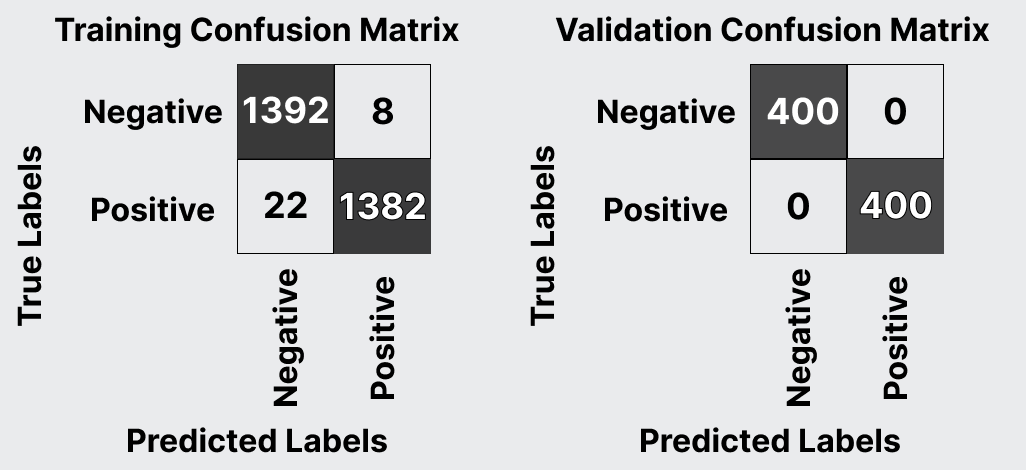
\includegraphics[scale=0.3]{gambar/bab4/tvcon1.png}
    \caption{Confussion Matrix Training dan Validasi Percobaan Pertama}
    \label{fig:tvcon1}
\end{figure}

\begin{figure} [H] \centering
    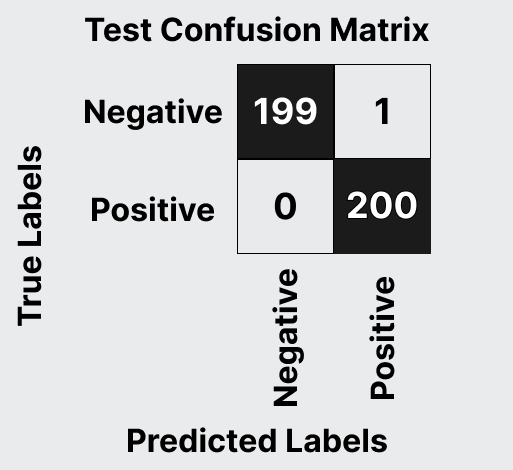
\includegraphics[scale=0.3]{gambar/bab4/testcon1.png}
    \caption{Confussion Matrix Testing Percobaan Pertama}
    \label{fig:testcon1}
\end{figure}

Hasil training yang cukup baik dari percobaan pertama dapat dilihat pula pada keberhasilannya dalam mengklasifikasikan gambar dengan tepat seperti yang dapat dilihat pada gambar berikut:

\begin{figure} [H] \centering
    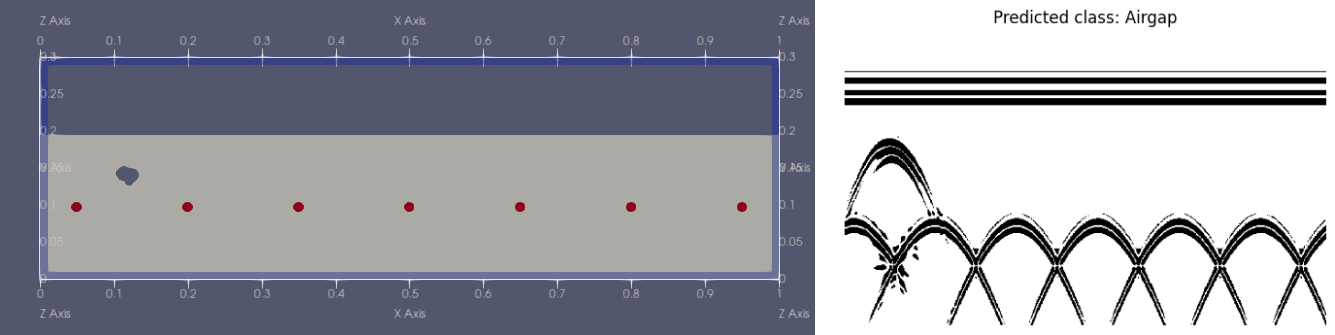
\includegraphics[scale=0.2]{gambar/bab4/Airgap 1999.png}
    \caption{Hasil Klasifikasi Percobaan Pertama 1}
\end{figure}

\begin{figure} [H] \centering
    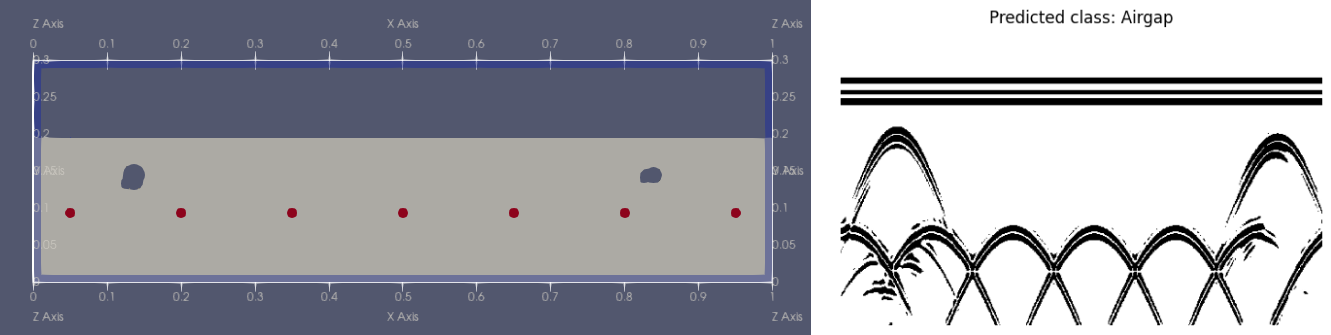
\includegraphics[scale=0.2]{gambar/bab4/Airgap 2000.png}
    \caption{Hasil Klasifikasi Percobaan Pertama 2}
\end{figure}

\begin{figure} [H] \centering
    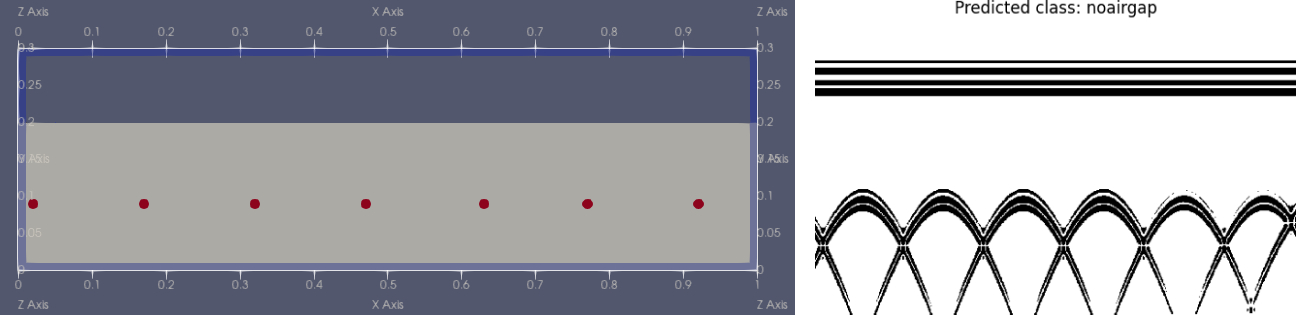
\includegraphics[scale=0.2]{gambar/bab4/Noarigap 1900.png}
    \caption{Hasil Klasifikasi Percobaan Pertama 3}
\end{figure}

\begin{figure} [H] \centering
    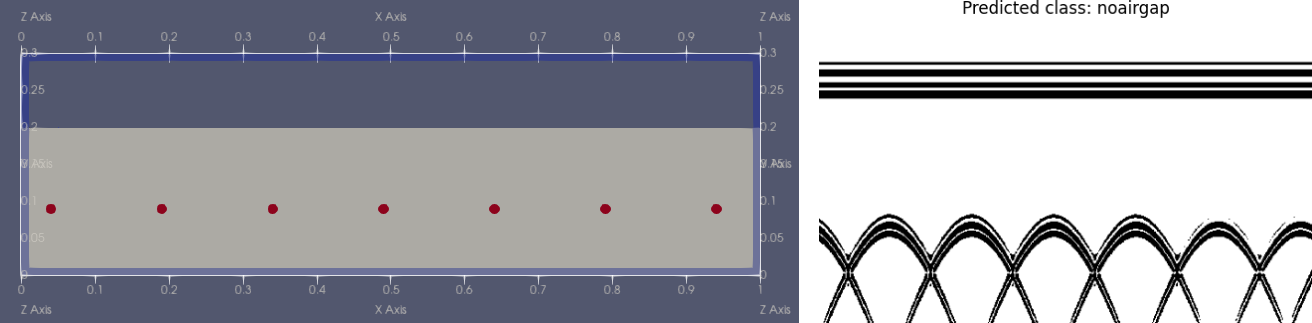
\includegraphics[scale=0.2]{gambar/bab4/Noairgap 2000.png}
    \caption{Hasil Klasifikasi Percobaan Pertama 4}
\end{figure}

\subsection{Percobaan Kedua}
Pada percobaan kedua, data yang digunakan untuk training, validation, dan testing masing-masing sebanyak 70\%, 15\%, dan 15\%. Hasil klasifikasi menggunakan CNN 2-Dimensi pada percobaan kedua mendapatkan tingkat akurasi training sebesar 0.9964 dengan training loss sebesar 0.0103. Sementara itu, didapatkan tingkat akurasi validasi sebesar 1.0 dengan valiation loss sebesar 2.0294e-04. Berikut ini adalah grafik model accuracy dan model loss pada percobaan kedua yang dapat dilihat pada Gambar \ref{fig:trainres2}.

\begin{figure} [H] \centering
    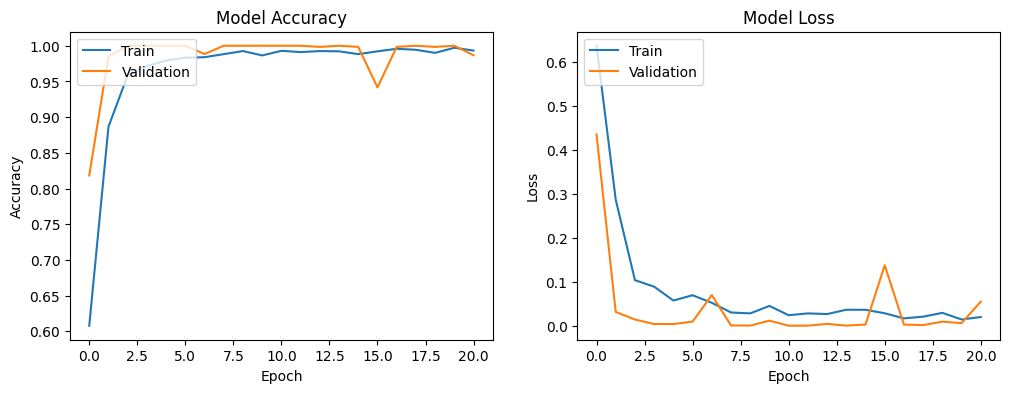
\includegraphics[scale=0.5]{gambar/bab4/trainres2.png}
    \caption{Grafik Akurasi dan Loss Model Percobaan Kedua}
    \label{fig:trainres2}
\end{figure}

Selain itu, didapatkan pula hasil confusion matrix dari data training, validation, dan testing pada percobaan kedua yang masing-masing dapat dilihat pada Gambar \ref{fig:tvcon2} dan \ref{fig:testcon2}. Dari hasil tersebut, dapat dilihat bahwa hasil klasifikasi menggunakan CNN 2-Dimensi pada percobaan kedua memiliki tingkat akurasi yang cukup tinggi. Hal ini didukung dengan nilai f1 score pada data training sebesar 0.99714893, validation sebesar 1.0, dan testing sebesar 1.0. Inference time yang didapatkan pada percobaan kedua untuk data training sebanyak 2800 data adalah 80 detik (285ms/step), untuk data validation sebanyak 600 data adalah 7 detik (115ms/step), dan untuk data testing sebanyak 600 data adalah 8 detik (128ms/step).

\begin{figure} [H] \centering
    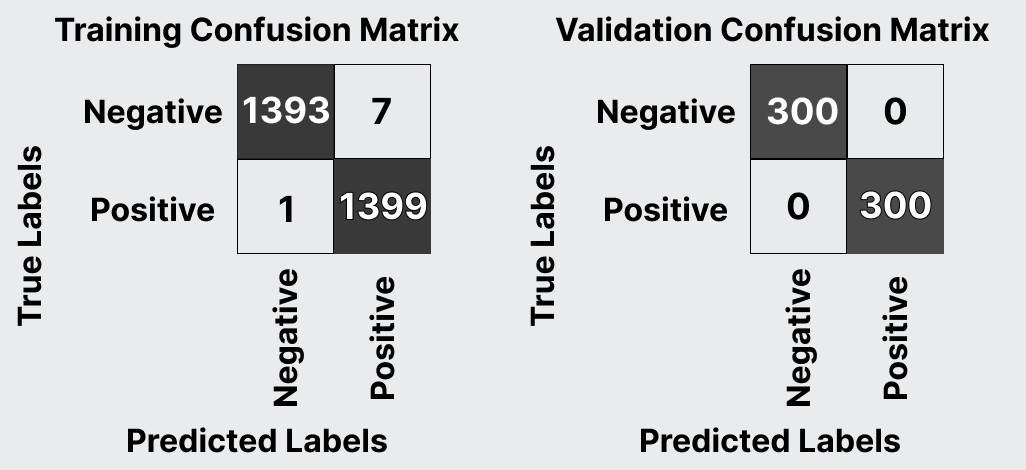
\includegraphics[scale=0.3]{gambar/bab4/tvcon2.png}
    \caption{Confussion Matrix Training dan Validasi Percobaan Kedua}
    \label{fig:tvcon2}
\end{figure}

\begin{figure} [H] \centering
    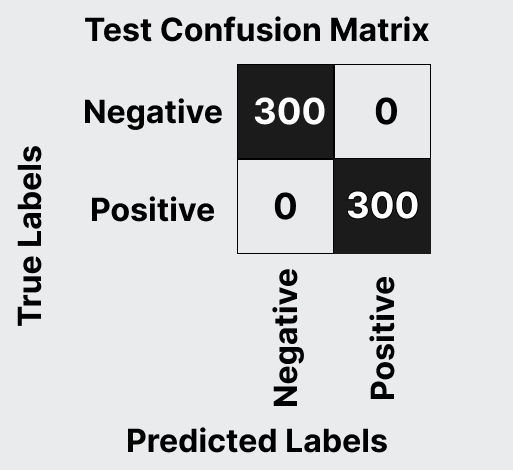
\includegraphics[scale=0.3]{gambar/bab4/testcon2.png}
    \caption{Confussion Matrix Testing Percobaan Kedua}
    \label{fig:testcon2}
\end{figure}

Hasil training yang cukup baik dari percobaan kedua dapat dilihat pula pada keberhasilannya dalam mengklasifikasikan gambar dengan tepat seperti yang dapat dilihat pada gambar berikut:

\begin{figure} [H] \centering
    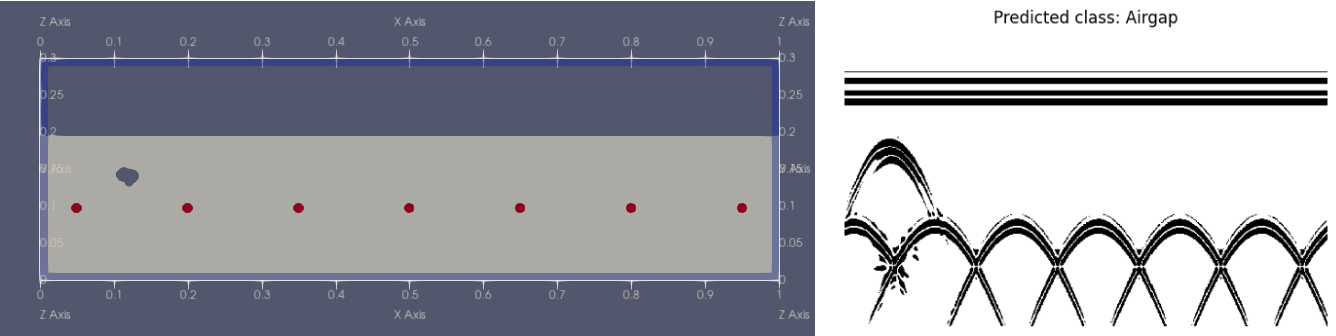
\includegraphics[scale=0.2]{gambar/bab4/Airgap 19992.png}
    \caption{Hasil Klasifikasi Percobaan Kedua 1}
\end{figure}

\begin{figure} [H] \centering
    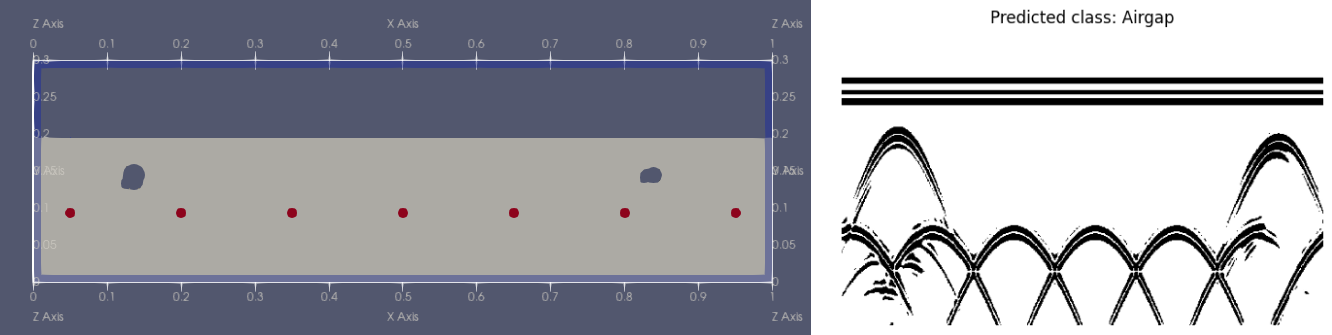
\includegraphics[scale=0.2]{gambar/bab4/Airgap 20002.png}
    \caption{Hasil Klasifikasi Percobaan Kedua 2}
\end{figure}

\begin{figure} [H] \centering
    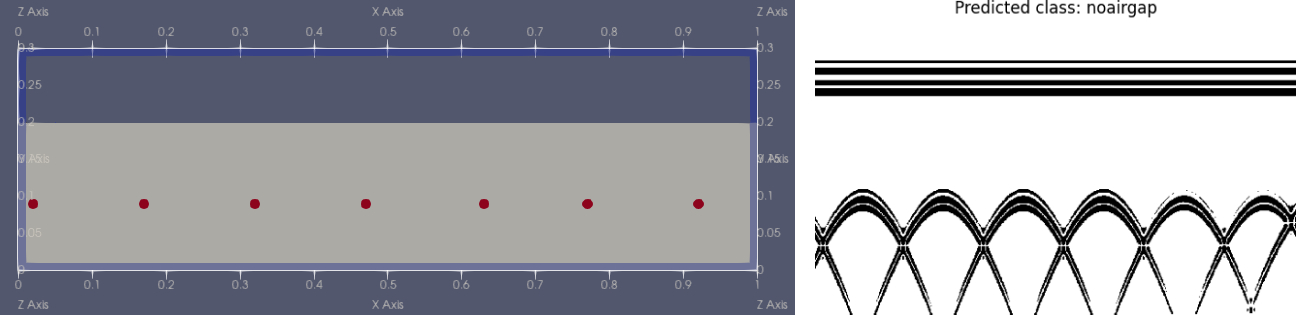
\includegraphics[scale=0.2]{gambar/bab4/Noarigap 19002.png}
    \caption{Hasil Klasifikasi Percobaan Kedua 3}
\end{figure}

\begin{figure} [H] \centering
    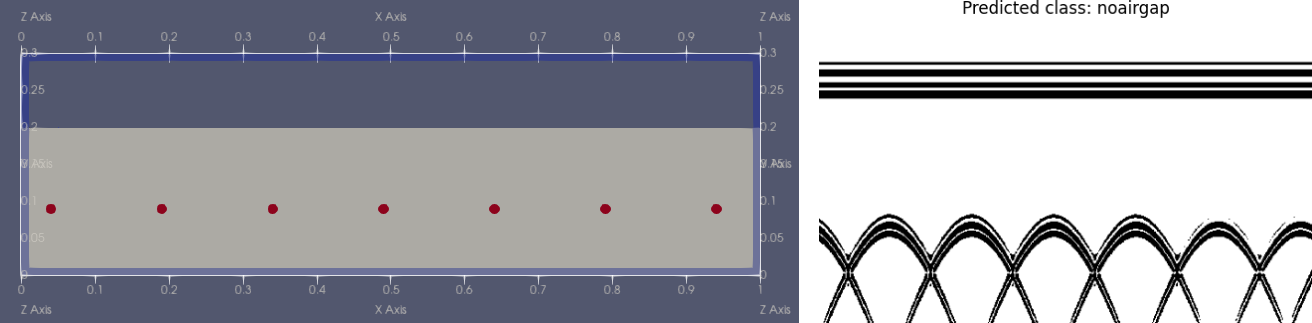
\includegraphics[scale=0.2]{gambar/bab4/Noairgap 20002.png}
    \caption{Hasil Klasifikasi Percobaan Kedua 4}
\end{figure}

\subsection{Percobaan Ketiga}
Pada percobaan ketiga, data yang digunakan untuk training, validation, dan testing masing-masing sebanyak 60\%, 20\%, dan 20\%. Hasil klasifikasi menggunakan CNN 2-Dimensi pada percobaan ketiga mendapatkan tingkat akurasi training sebesar 0.9946 dengan training loss sebesar 0.0147. Sementara itu, didapatkan tingkat akurasi validasi sebesar 1.0 dengan valiation loss sebesar 1.1496e-04. Berikut ini adalah grafik model accuracy dan model loss pada percobaan ketiga yang dapat dilihat pada Gambar \ref{fig:trainres3}.

\begin{figure} [H] \centering
    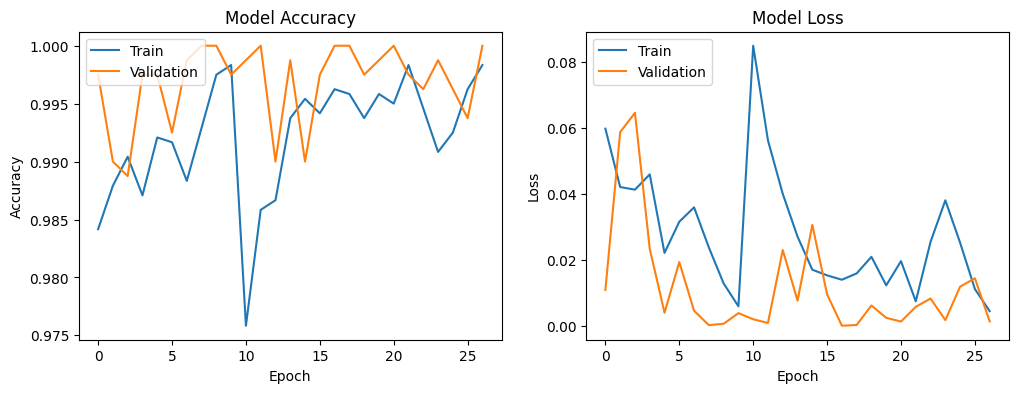
\includegraphics[scale=0.5]{gambar/bab4/trainres3.png}
    \caption{Grafik Akurasi dan Loss Model Percobaan Ketiga}
    \label{fig:trainres3}
\end{figure}

Meskipun pada hasil training, model memiliki hasil yang baik, grafik hasil training menunjukan training yang tidak begitu baik dan mengindikasikan overfitting dengan adanya spiking. Tidak dipungkiri bahwa hal ini dapat terjadi karena pada salah satu kelas dataset yakni noairgap, kelas tersebut memiliki data yang hampir serupa satu sama lain. Selain itu, didapatkan pula hasil confusion matrix dari data training, validation, dan testing pada percobaan ketiga yang masing-masing dapat dilihat pada Gambar \ref{fig:tvcon3} dan \ref{fig:testcon3}. Dari hasil tersebut, dapat dilihat bahwa hasil klasifikasi menggunakan CNN 2-Dimensi pada percobaan ketiga memiliki tingkat akurasi yang baik. Meskipun pada confusion matriks data training dan valiasi masih menunjukkan kesalahan, namun pada data testing menunjukkan keakuratan yang baik. Hal ini didukung dengan nilai f1 score pada data training sebesar 0.99502486, validation sebesar 1.0, dan testing sebesar 1.0. Inference time yang didapatkan pada percobaan ketiga untuk data training sebanyak 2400 data adalah 72 detik (301ms/step), untuk data validation sebanyak 800 data adalah 9 detik (114ms/step), dan untuk data testing sebanyak 800 data adalah 115 detik (1s/step).

\begin{figure} [H] \centering
    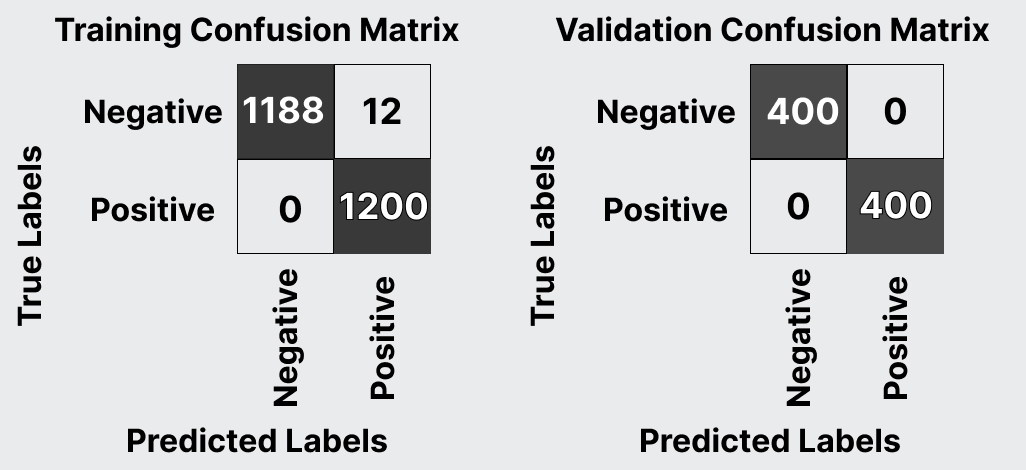
\includegraphics[scale=0.3]{gambar/bab4/tvcon3.png}
    \caption{Confussion Matrix Training dan Validasi Percobaan Ketiga}
    \label{fig:tvcon3}
\end{figure}

\begin{figure} [H] \centering
    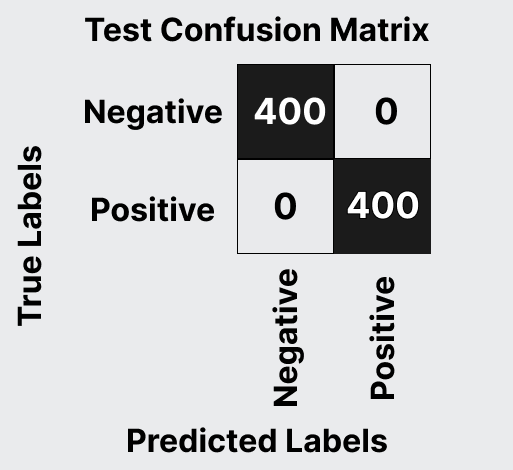
\includegraphics[scale=0.3]{gambar/bab4/testcon3.png}
    \caption{Confussion Matrix Testing Percobaan Ketiga}
    \label{fig:testcon3}
\end{figure}

Hasil training yang cukup baik dari percobaan ketiga dapat dilihat pula pada keberhasilannya dalam mengklasifikasikan gambar dengan tepat seperti yang dapat dilihat pada gambar berikut:

\begin{figure} [H] \centering
    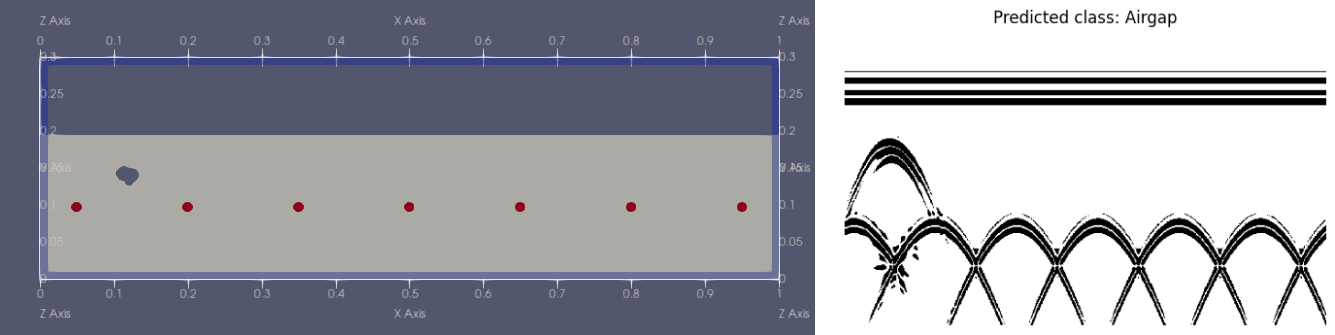
\includegraphics[scale=0.2]{gambar/bab4/Airgap 19993.png}
    \caption{Hasil Klasifikasi Percobaan Ketiga 1}
\end{figure}

\begin{figure} [H] \centering
    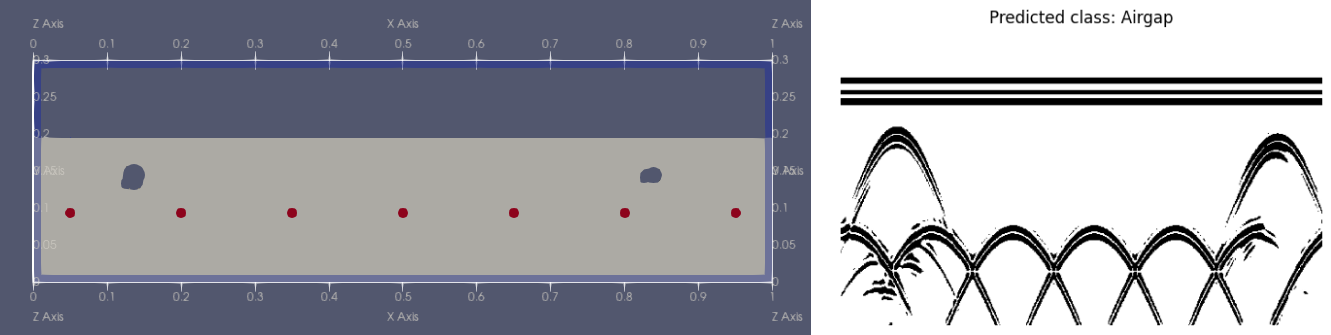
\includegraphics[scale=0.2]{gambar/bab4/Airgap 20003.png}
    \caption{Hasil Klasifikasi Percobaan Ketiga 2}
\end{figure}

\begin{figure} [H] \centering
    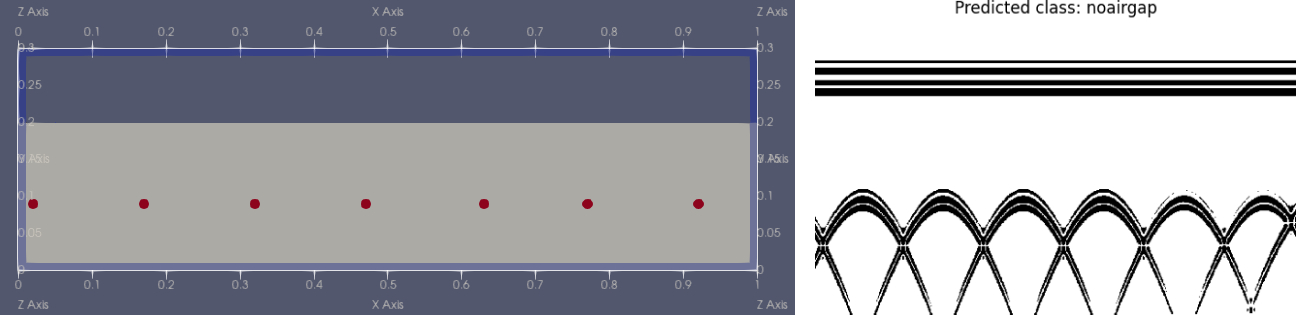
\includegraphics[scale=0.2]{gambar/bab4/Noarigap 19003.png}
    \caption{Hasil Klasifikasi Percobaan Ketiga 3}
\end{figure}

\begin{figure} [H] \centering
    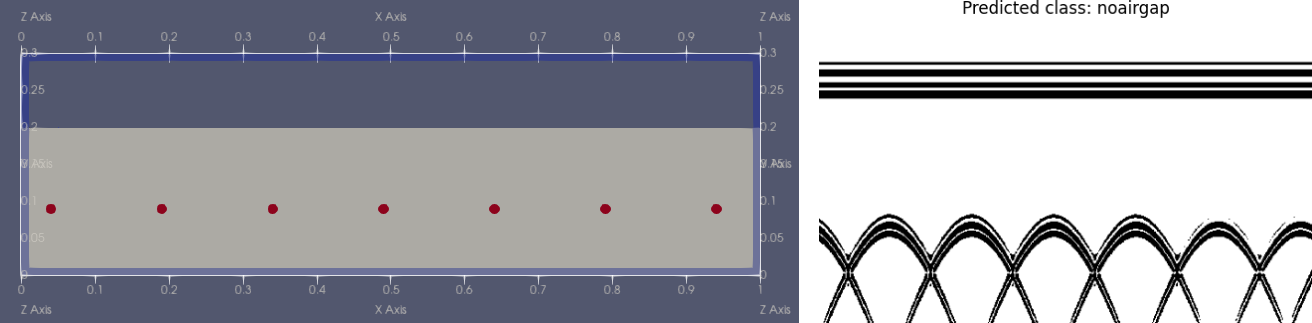
\includegraphics[scale=0.2]{gambar/bab4/Noairgap 20003.png}
    \caption{Hasil Klasifikasi Percobaan Ketiga 4}
\end{figure}

\subsection{Percobaan Keempat}
Pada percobaan keempat, data yang digunakan untuk training, validation, dan testing masing-masing sebanyak 70\%, 15\%, dan 15\%. Selain itu, ditambahkan variasi untuk kode CNN 2-Dimensi dengan menambahkan BatchNormalization setelah setiap layer Conv2D. Hasil klasifikasi menggunakan CNN 2-Dimensi pada percobaan keempat mendapatkan tingkat akurasi training sebesar 0.9621 dengan training loss sebesar 0.1670. Sementara itu, didapatkan tingkat akurasi validasi sebesar 0.9833 dengan valiation loss sebesar 0.1061. Berikut ini adalah grafik model accuracy dan model loss pada percobaan keempat yang dapat dilihat pada Gambar \ref{fig:trainres4}.

\begin{figure} [H] \centering
    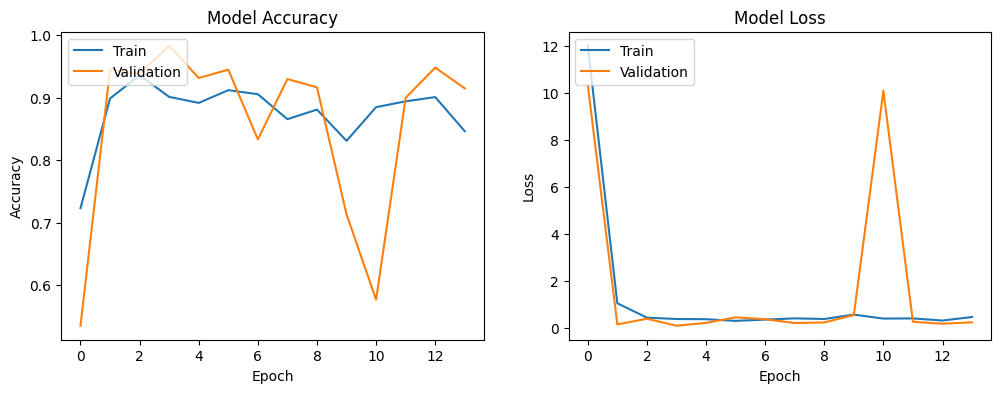
\includegraphics[scale=0.5]{gambar/bab4/trainres4.png}
    \caption{Grafik Akurasi dan Loss Model Percobaan Keempat}
    \label{fig:trainres4}
\end{figure}

Berdasarkan grafik hasil training, meskipun hasil memiliki tingkat keakurasian yang baik, grafik menunjukkan perilaku yang tidak wajar dimana terjadi spiking yang tinggi. Hal ini dapat terjadi karena pada salah satu kelas dataset yakni noairgap, kelas tersebut memiliki data yang hampir serupa satu sama lain. Penyebab lain dapat bersumber dari perubahan struktur layer CNN 2-Dimensis yang digunakan. Selain itu, didapatkan pula hasil confusion matrix dari data training, validation, dan testing pada percobaan keempat yang masing-masing dapat dilihat pada Gambar \ref{fig:tvcon4} dan \ref{fig:testcon4}. Dari hasil tersebut, dapat dilihat bahwa hasil klasifikasi menggunakan CNN 2-Dimensi pada percobaan keempat memiliki tingkat akurasi sedang. Hal ini didukung dengan hasil confusion matrix pada data training, validasi, dan testing yang memiliki error yang lebih banyak dibandingkan dengan percobaan yang lain. Nilai f1 score yang didapatkan pada data training sebesar 0.961155, validation sebesar 0.98360646, dan testing sebesar 0.9803921. Inference time yang didapatkan pada percobaan keempat untuk data training sebanyak 2800 data adalah 79 detik (281ms/step), untuk data validation sebanyak 600 data adalah 10 detik (162ms/step), dan untuk data testing sebanyak 600 data adalah 130 detik (2s/step).

\begin{figure} [H] \centering
    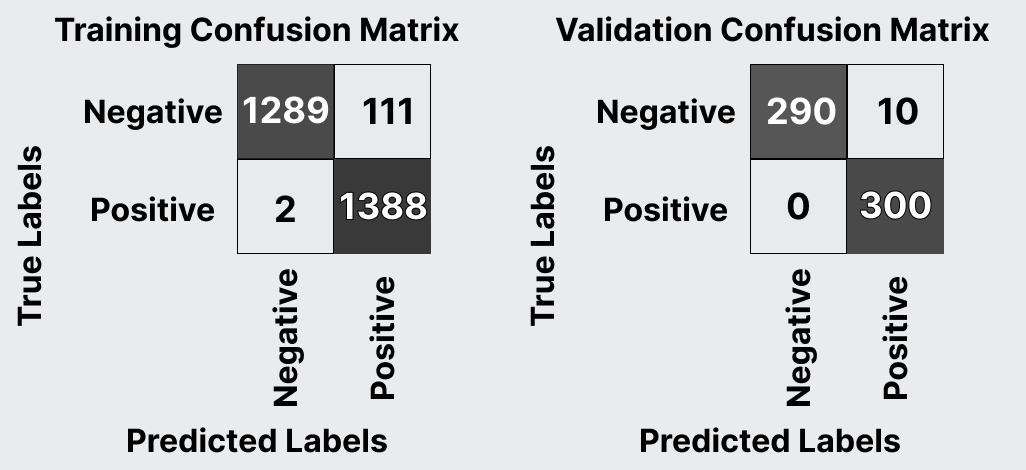
\includegraphics[scale=0.3]{gambar/bab4/tvcon4.png}
    \caption{Confussion Matrix Training dan Validasi Percobaan Keempat}
    \label{fig:tvcon4}
\end{figure}

\begin{figure} [H] \centering
    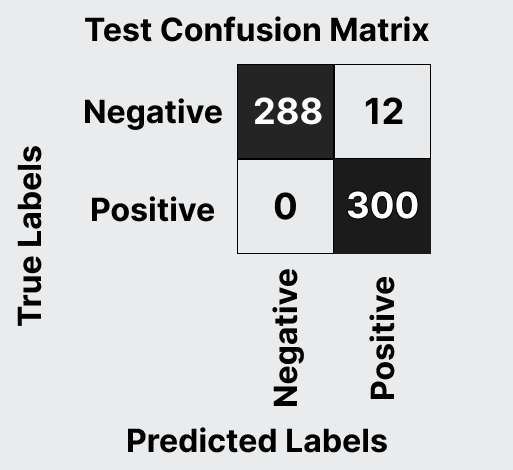
\includegraphics[scale=0.3]{gambar/bab4/testcon4.png}
    \caption{Confussion Matrix Testing Percobaan Keempat}
    \label{fig:testcon4}
\end{figure}

Hasil training yang cukup baik dari percobaan keempat dapat dilihat pula pada keberhasilannya dalam mengklasifikasikan gambar dengan tepat seperti yang dapat dilihat pada gambar berikut:

\begin{figure} [H] \centering
    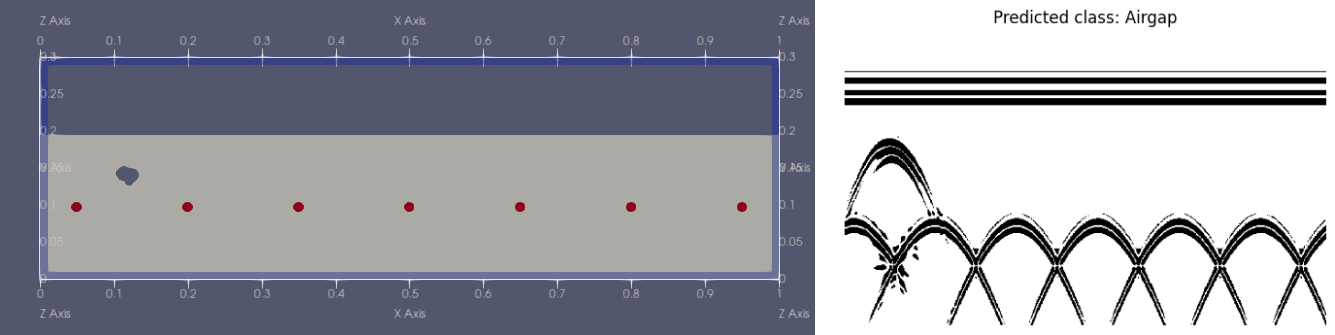
\includegraphics[scale=0.2]{gambar/bab4/Airgap 19994.png}
    \caption{Hasil Klasifikasi Percobaan Keempat 1}
\end{figure}

\begin{figure} [H] \centering
    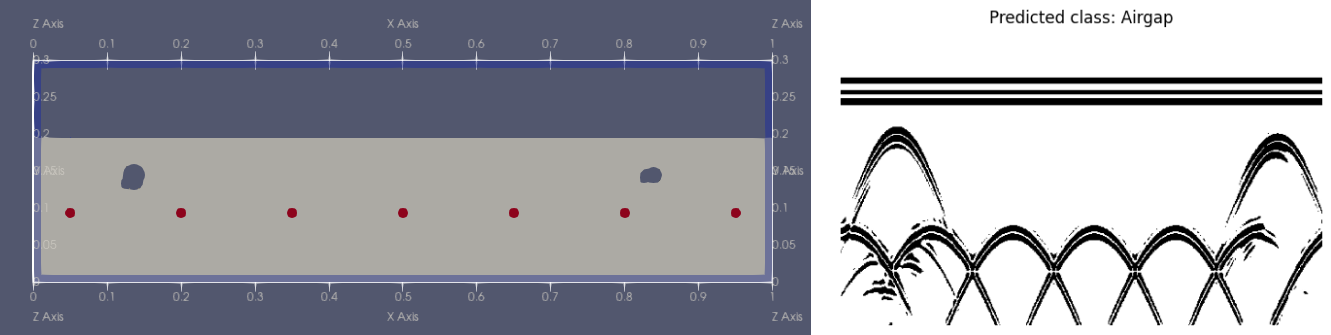
\includegraphics[scale=0.2]{gambar/bab4/Airgap 20004.png}
    \caption{Hasil Klasifikasi Percobaan Keempat 2}
\end{figure}

\begin{figure} [H] \centering
    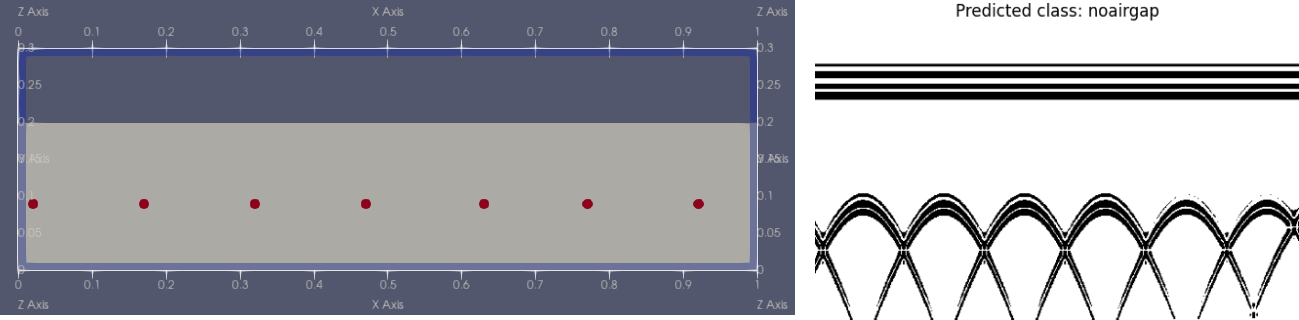
\includegraphics[scale=0.2]{gambar/bab4/Noarigap 19004.png}
    \caption{Hasil Klasifikasi Percobaan Keempat 3}
\end{figure}

\begin{figure} [H] \centering
    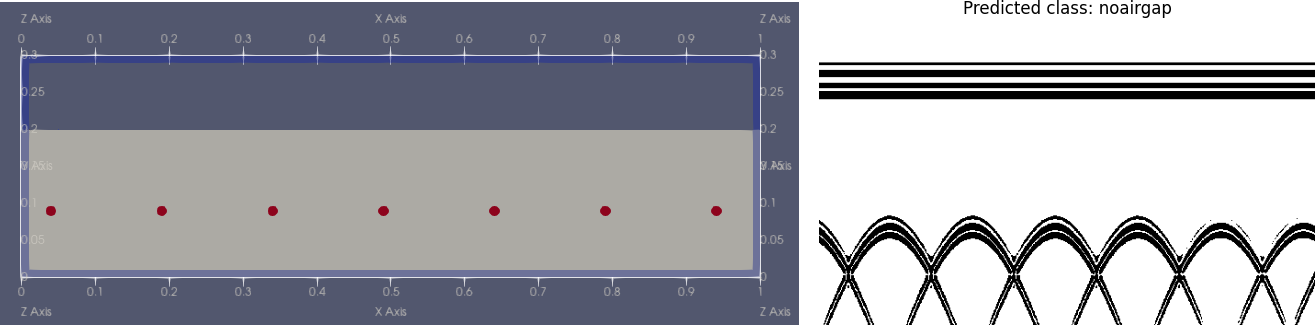
\includegraphics[scale=0.2]{gambar/bab4/Noairgap 20004.png}
    \caption{Hasil Klasifikasi Percobaan Keempat 4}
\end{figure}

\subsection{Percobaan Kelima}
Pada percobaan kelima, data yang digunakan untuk training, validation, dan testing masing-masing sebanyak 70\%, 15\%, dan 15\%. Pada percobaan ini, ditambahkan variasi untuk kode CNN 2-Dimensi dengan mengurangi jumlah layer Conv2D menjadi dua dan layer Dense menjadi 1. Layer Conv2D berawal dari 32 dan berakhir di 64 dengan MaxPooling dan BatchNormalization yang sama dengan percobaan keempat. Hasil klasifikasi menggunakan CNN 2-Dimensi pada percobaan kelima mendapatkan tingkat akurasi training sebesar 0.9154 dengan training loss sebesar 0.2236. Sementara itu, didapatkan tingkat akurasi validasi sebesar 0.9867 dengan valiation loss sebesar 0.0336. Berikut ini adalah grafik model accuracy dan model loss pada percobaan kelima yang dapat dilihat pada Gambar \ref{fig:trainres5}.

\begin{figure} [H] \centering
    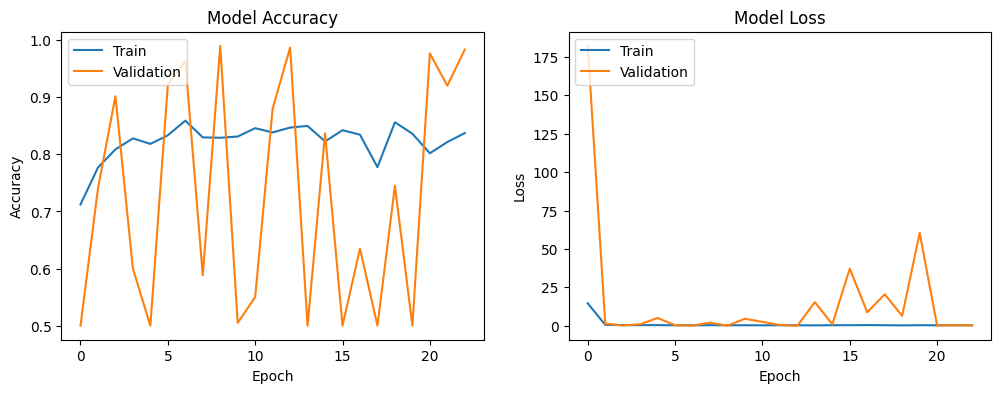
\includegraphics[scale=0.5]{gambar/bab4/trainres5.png}
    \caption{Grafik Akurasi dan Loss Model Percobaan Kelima}
    \label{fig:trainres5}
\end{figure}

Berdasarkan grafik hasil training, meskipun hasil memiliki tingkat keakurasian yang lebih rendah dibandingkan percobaan sebelumnya, grafik menunjukkan perilaku yang tidak wajar dimana grafik menunjukan nilai yang tinggi kemudian rendah berulang kali. Hal ini dapat terjadi karena pada salah satu kelas dataset yakni noairgap, kelas tersebut memiliki data yang hampir serupa satu sama lain. Penyebab lain dapat bersumber dari perubahan struktur layer CNN 2-Dimensis yang digunakan. Selain itu, didapatkan pula hasil confusion matrix dari data training, validation, dan testing pada percobaan kelima yang masing-masing dapat dilihat pada Gambar \ref{fig:tvcon5} dan \ref{fig:testcon5}. Dari hasil tersebut, dapat dilihat bahwa hasil klasifikasi menggunakan CNN 2-Dimensi pada percobaan kelima terjadi penurunan dalam hal tingkat akurasi. Didapatkan nilai f1 score pada data training sebesar 0.92211217, validation sebesar 0.98684204, dan testing sebesar 0.98360646. Inference time yang didapatkan pada percobaan kelima untuk data training sebanyak 2800 data adalah 85 detik (304ms/step), untuk data validation sebanyak 600 data adalah 8 detik (125ms/step), dan untuk data testing sebanyak 600 data adalah 83 detik (1s/step).

\begin{figure} [H] \centering
    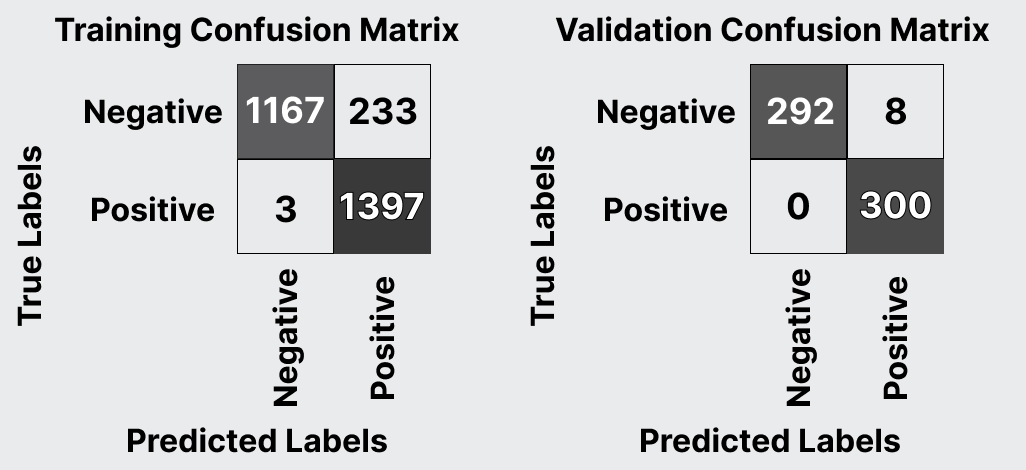
\includegraphics[scale=0.3]{gambar/bab4/tvcon5.png}
    \caption{Confussion Matrix Training dan Validasi Percobaan Kelima}
    \label{fig:tvcon5}
\end{figure}

\begin{figure} [H] \centering
    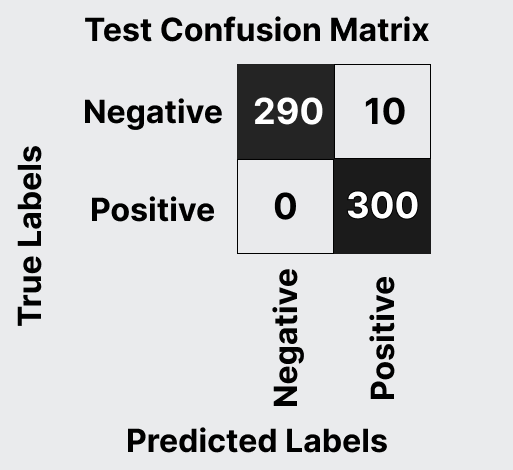
\includegraphics[scale=0.3]{gambar/bab4/testcon5.png}
    \caption{Confussion Matrix Testing Percobaan Kelima}
    \label{fig:testcon5}
\end{figure}

Hasil training yang cukup baik dari percobaan kelima dapat dilihat pula pada keberhasilannya dalam mengklasifikasikan gambar dengan tepat seperti yang dapat dilihat pada gambar berikut:

\begin{figure} [H] \centering
    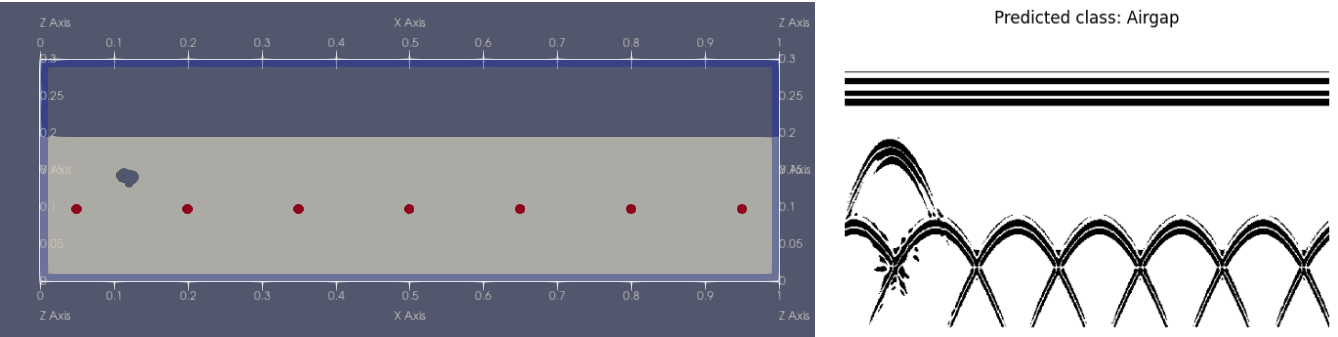
\includegraphics[scale=0.2]{gambar/bab4/Airgap 19995.png}
    \caption{Hasil Klasifikasi Percobaan Kelima 1}
\end{figure}

\begin{figure} [H] \centering
    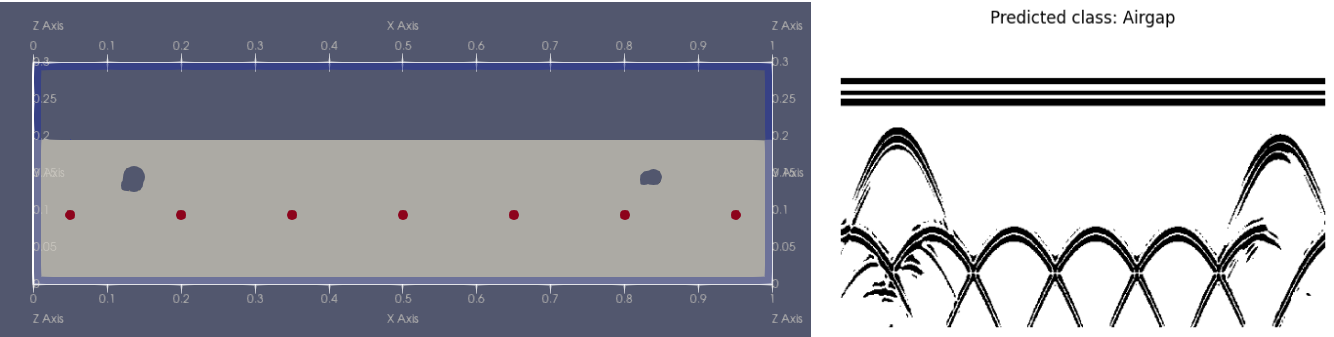
\includegraphics[scale=0.2]{gambar/bab4/Airgap 20005.png}
    \caption{Hasil Klasifikasi Percobaan Kelima 2}
\end{figure}

\begin{figure} [H] \centering
    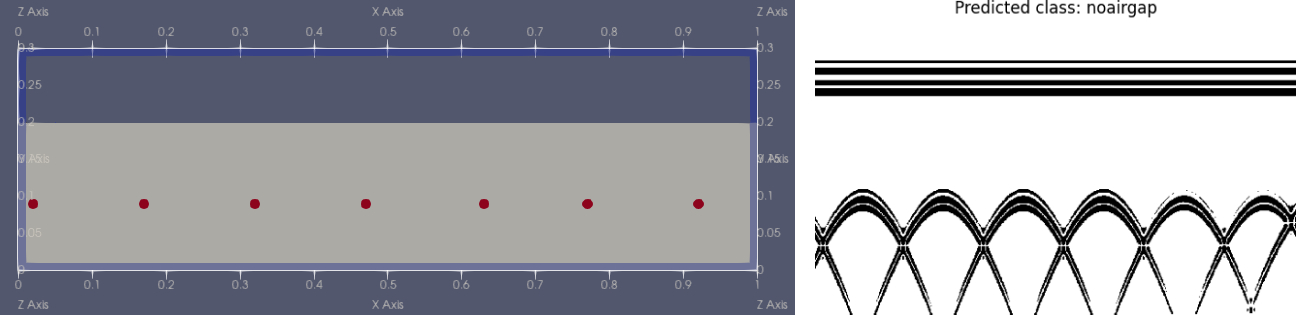
\includegraphics[scale=0.2]{gambar/bab4/Noarigap 19005.png}
    \caption{Hasil Klasifikasi Percobaan Kelima 3}
\end{figure}

\begin{figure} [H] \centering
    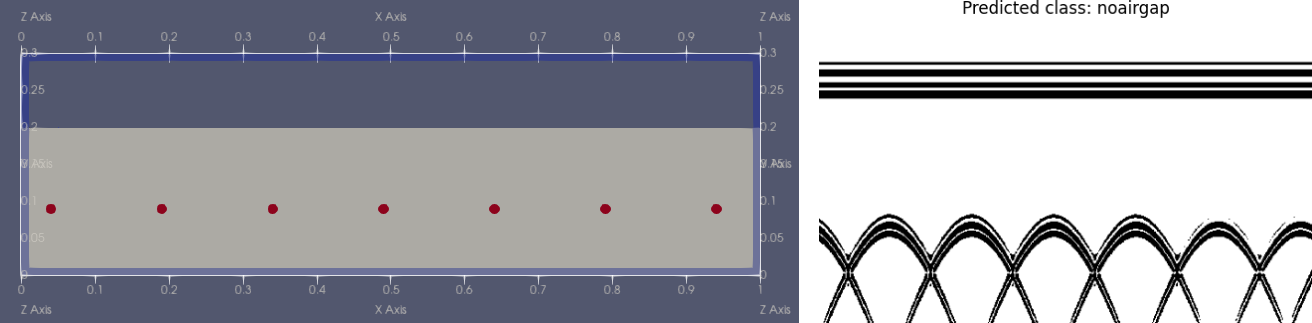
\includegraphics[scale=0.2]{gambar/bab4/Noairgap 20005.png}
    \caption{Hasil Klasifikasi Percobaan Kelima 4}
\end{figure}

\subsection{Percobaan Keenam}
Pada percobaan keenam, data yang digunakan untuk training, validation, dan testing masing-masing sebanyak 70\%, 15\%, dan 15\%. Pada percobaan ini, ditambahkan variasi untuk kode CNN 2-Dimensi dengan menjadikan struktur CNN 2-Dimensi hanya memiliki 3 layer Conv2D tanpa BatchNormalization, masih memiliki MaxPooling yang sama namun layer Conv2D memiliki parameter tambahan yakni padding yang nilainya diatur menjadi 'same' dengan layer Conv2D bermula dari 32 dan berakhir pada 128. Selain itu, ditambahkan dropout layer senilai 0.25 sebelum memasuki flatten layer dan ditambahkan 1 Dense layer setelahnya. Hasil klasifikasi menggunakan CNN 2-Dimensi pada percobaan keenam mendapatkan tingkat akurasi training sebesar 0.9993 dengan training loss sebesar 0.0028. Sementara itu, didapatkan tingkat akurasi validasi sebesar 1.0 dengan valiation loss sebesar 4.2127e-06. Berikut ini adalah grafik model accuracy dan model loss pada percobaan keenam yang dapat dilihat pada Gambar \ref{fig:trainres6}.

\begin{figure} [H] \centering
    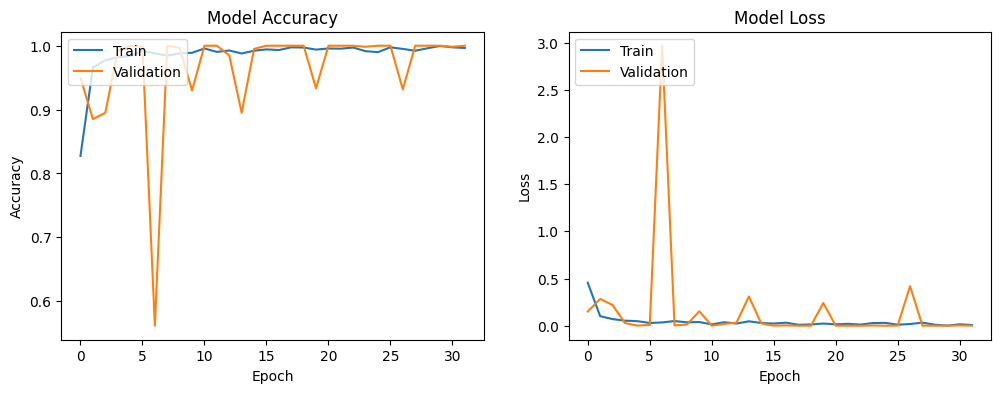
\includegraphics[scale=0.5]{gambar/bab4/trainres6.png}
    \caption{Grafik Akurasi dan Loss Model Percobaan Keenam}
    \label{fig:trainres6}
\end{figure}

Berdasarkan grafik hasil training, meskipun hasil memiliki tingkat keakurasian yang perlahan-lahan membaik dibandingkan percobaan sebelumnya, grafik menunjukkan perilaku yang tidak wajar dimana grafik menunjukan spiking yang tinggi. Hal ini dapat terjadi karena pada salah satu kelas dataset yakni noairgap, kelas tersebut memiliki data yang hampir serupa satu sama lain. Selain itu, didapatkan pula hasil confusion matrix dari data training, validation, dan testing pada percobaan keenam yang masing-masing dapat dilihat pada Gambar \ref{fig:tvcon6} dan \ref{fig:testcon6}. Dari hasil tersebut, dapat dilihat bahwa hasil klasifikasi menggunakan CNN 2-Dimensi pada percobaan keenam memiliki tingkat akurasi yang cukup tinggi. Hal ini didukung dengan nilai f1 score pada data training sebesar 0.9985734, validation sebesar 1.0, dan testing sebesar 1.0. Inference time yang didapatkan pada percobaan keenam untuk data training sebanyak 2800 data adalah 76 detik (269ms/step), untuk data validation sebanyak 600 data adalah 7 detik (119ms/step), dan untuk data testing sebanyak 600 data adalah 97 detik (2s/step).

\begin{figure} [H] \centering
    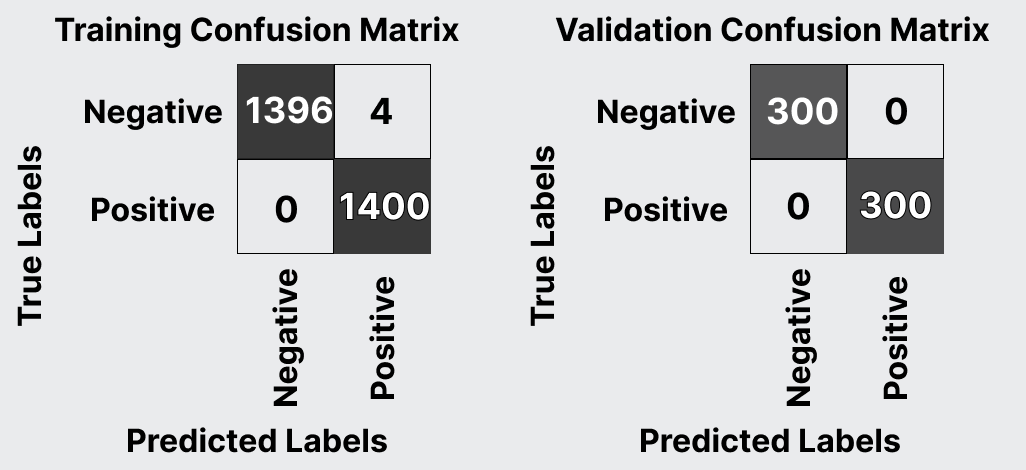
\includegraphics[scale=0.3]{gambar/bab4/tvcon6.png}
    \caption{Confussion Matrix Training dan Validasi Percobaan Keenam}
    \label{fig:tvcon6}
\end{figure}

\begin{figure} [H] \centering
    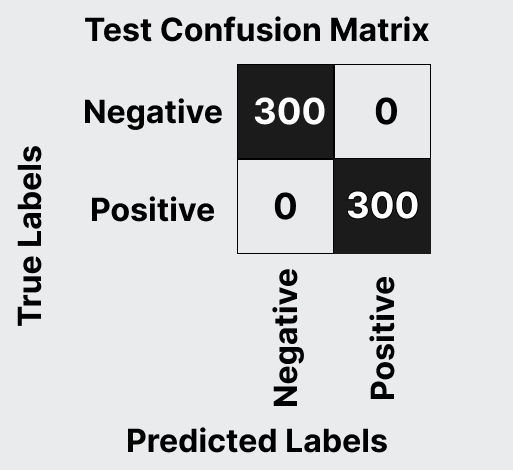
\includegraphics[scale=0.3]{gambar/bab4/testcon6.png}
    \caption{Confussion Matrix Testing Percobaan Keenam}
    \label{fig:testcon6}
\end{figure}

Hasil training yang cukup baik dari percobaan keenam dapat dilihat pula pada keberhasilannya dalam mengklasifikasikan gambar dengan tepat seperti yang dapat dilihat pada gambar berikut:

\begin{figure} [H] \centering
    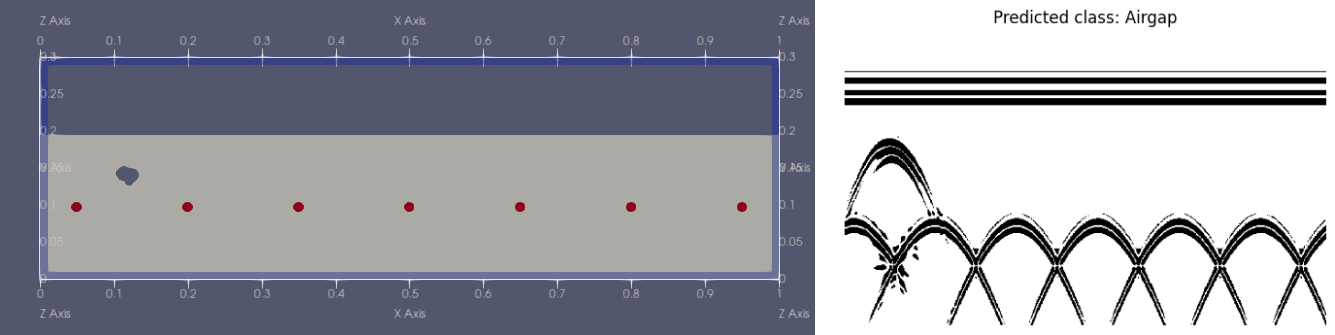
\includegraphics[scale=0.2]{gambar/bab4/Airgap 19996.png}
    \caption{Hasil Klasifikasi Percobaan Keenam 1}
\end{figure}

\begin{figure} [H] \centering
    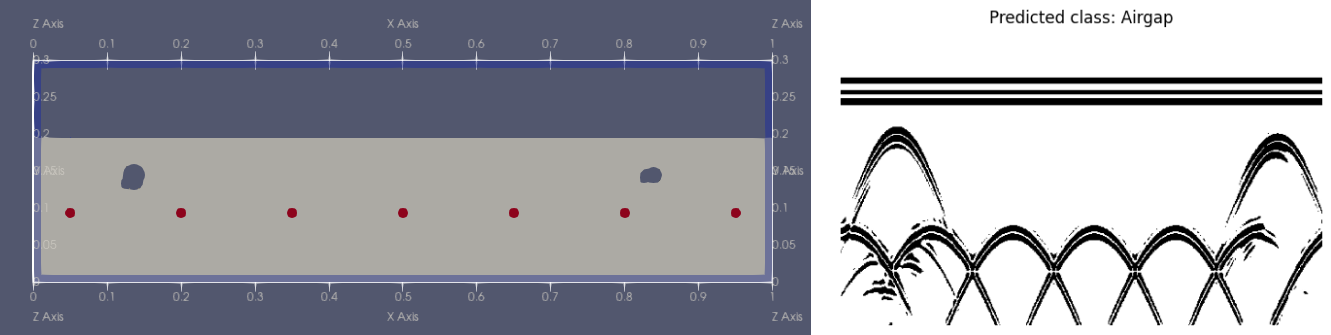
\includegraphics[scale=0.2]{gambar/bab4/Airgap 20006.png}
    \caption{Hasil Klasifikasi Percobaan Keenam 2}
\end{figure}

\begin{figure} [H] \centering
    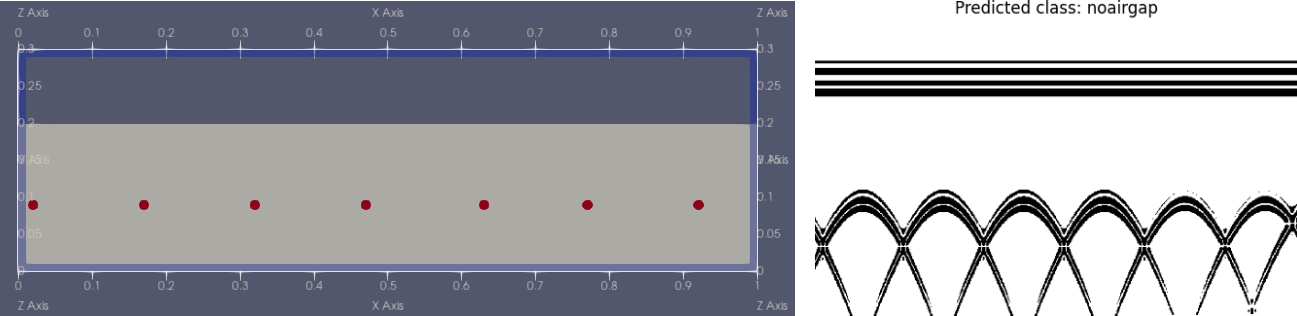
\includegraphics[scale=0.2]{gambar/bab4/Noarigap 19006.png}
    \caption{Hasil Klasifikasi Percobaan Keenam 3}
\end{figure}

\begin{figure} [H] \centering
    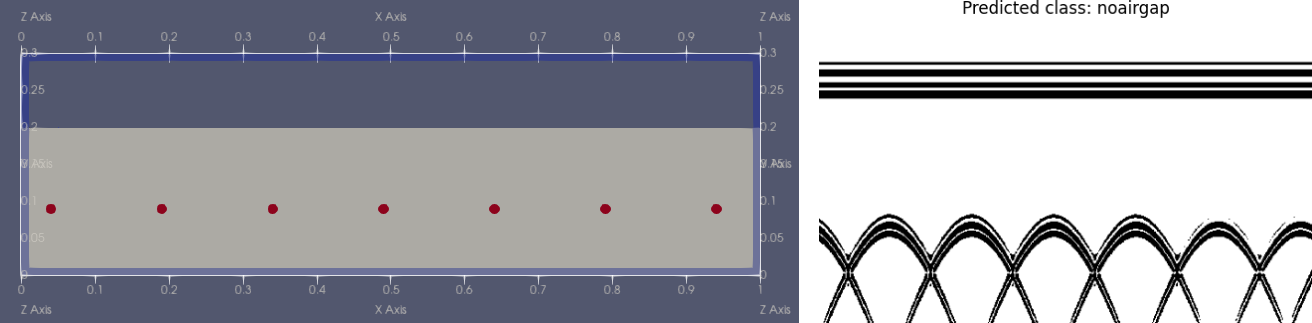
\includegraphics[scale=0.2]{gambar/bab4/Noairgap 20006.png}
    \caption{Hasil Klasifikasi Percobaan Keenam 4}
\end{figure}

Dari semua percobaan diatas, dapat diketahui bahwa hasil terbaik didapatkan pada percobaan kedua. Meskipun semua percobaan memiliki hasil klasifikasi yang baik, percobaan kedua memiliki hasil metrics yang lebih baik dibandingkan dengan percobaan lainnya.

\subsection{Percobaan Ketujuh}
Pada percobaan Ketujuh, data yang digunakan untuk training, validation, dan testing masing-masing sebanyak 70\%, 15\%, dan 15\%. Pada percobaan ini, ditambahkan variasi untuk kode CNN 2-Dimensi dengan menjadikan struktur CNN 2-Dimensi memiliki 6 layer Conv2D dengan masih memiliki MaxPooling yang sama namun hanya pada empat layer pertama. Selain itu, model ini tidak menggunakan dropout layer serta sebelum memasuki flatten layer dan ditambahkan 1 Dense layer setelahnya. Hasil klasifikasi menggunakan CNN 2-Dimensi pada percobaan ketujuh mendapatkan tingkat akurasi training sebesar 0.9979 dengan training loss sebesar 0.0060. Sementara itu, didapatkan tingkat akurasi validasi sebesar 1.0 dengan valiation loss sebesar 1.7544e-04. Berikut ini adalah grafik model accuracy dan model loss pada percobaan ketujuh yang dapat dilihat pada Gambar \ref{fig:trainres7}.

\begin{figure} [H] \centering
    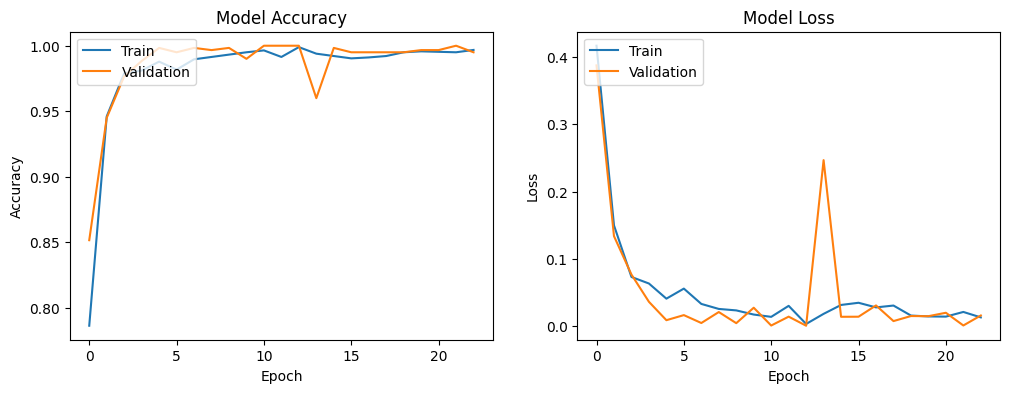
\includegraphics[scale=0.5]{gambar/bab4/trainres7.png}
    \caption{Grafik Akurasi dan Loss Model Percobaan Ketujuh}
    \label{fig:trainres7}
\end{figure}

Berdasarkan grafik hasil training, grafik menunjukkan perilaku yang tidak wajar dimana grafik menunjukan spiking yang tinggi. Hal ini dapat terjadi karena pada salah satu kelas dataset yakni noairgap, kelas tersebut memiliki data yang hampir serupa satu sama lain. Selain itu, didapatkan pula hasil confusion matrix dari data training, validation, dan testing pada percobaan ketujuh yang masing-masing dapat dilihat pada Gambar \ref{fig:tvcon7} dan \ref{fig:testcon7}. Dari hasil tersebut, dapat dilihat bahwa hasil klasifikasi menggunakan CNN 2-Dimensi pada percobaan ketujuh memiliki tingkat akurasi yang tinggi. Hal ini didukung dengan nilai f1 score pada data training sebesar 0.9985734, validation sebesar 1.0, dan testing sebesar 1.0. Inference time yang didapatkan pada percobaan ketujuh untuk data training sebanyak 2800 data adalah 76 detik (269ms/step), untuk data validation sebanyak 600 data adalah 6 detik (107ms/step), dan untuk data testing sebanyak 600 data adalah 81 detik (1s/step).

\begin{figure} [H] \centering
    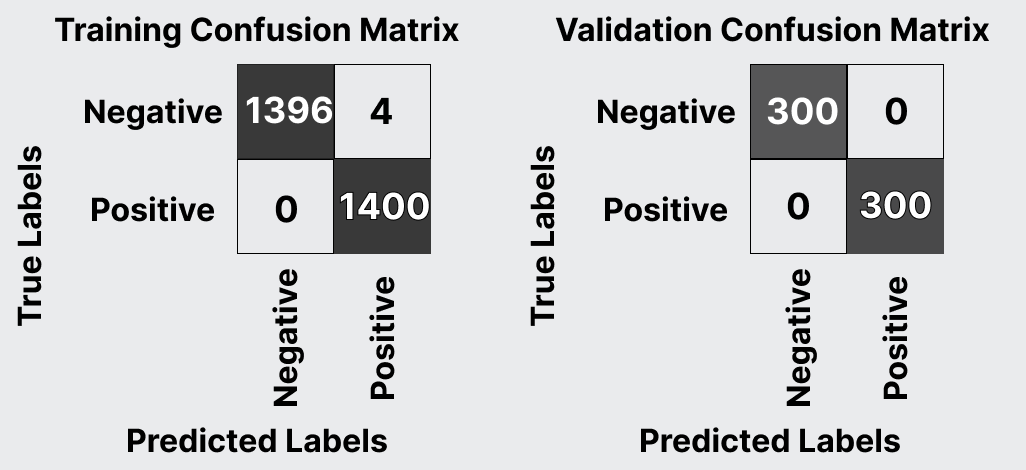
\includegraphics[scale=0.3]{gambar/bab4/tvcon7.png}
    \caption{Confussion Matrix Training dan Validasi Percobaan Ketujuh}
    \label{fig:tvcon7}
\end{figure}

\begin{figure} [H] \centering
    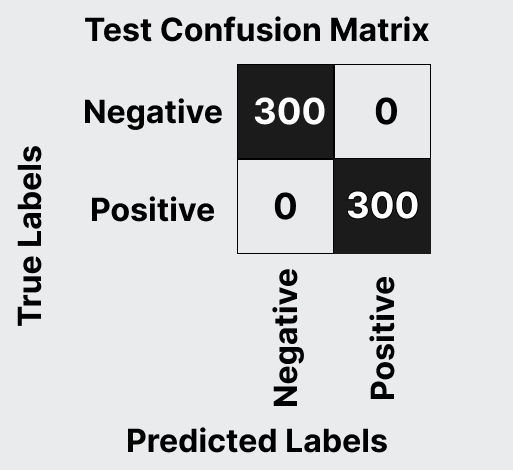
\includegraphics[scale=0.3]{gambar/bab4/testcon7.png}
    \caption{Confussion Matrix Testing Percobaan Ketujuh}
    \label{fig:testcon7}
\end{figure}

Hasil training yang cukup baik dari percobaan ketujuh dapat dilihat pula pada keberhasilannya dalam mengklasifikasikan gambar dengan tepat seperti yang dapat dilihat pada gambar berikut:

\begin{figure} [H] \centering
    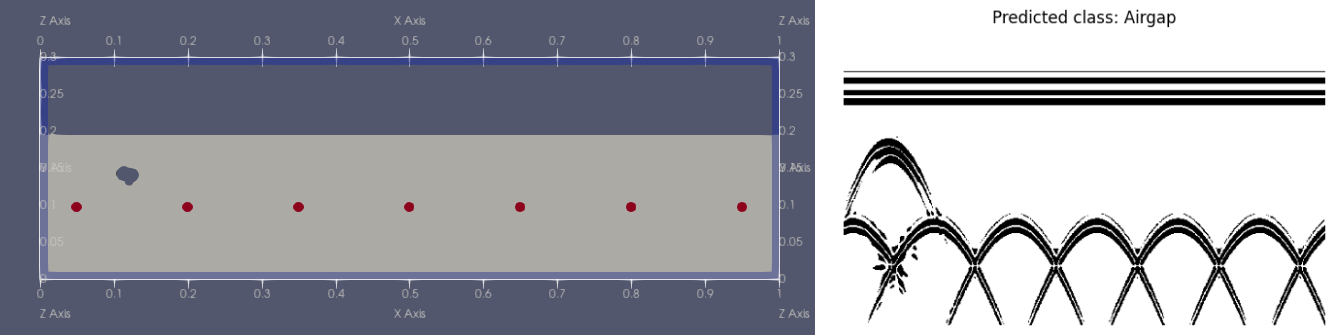
\includegraphics[scale=0.2]{gambar/bab4/Airgap 19997.png}
    \caption{Hasil Klasifikasi Percobaan Ketujuh 1}
\end{figure}

\begin{figure} [H] \centering
    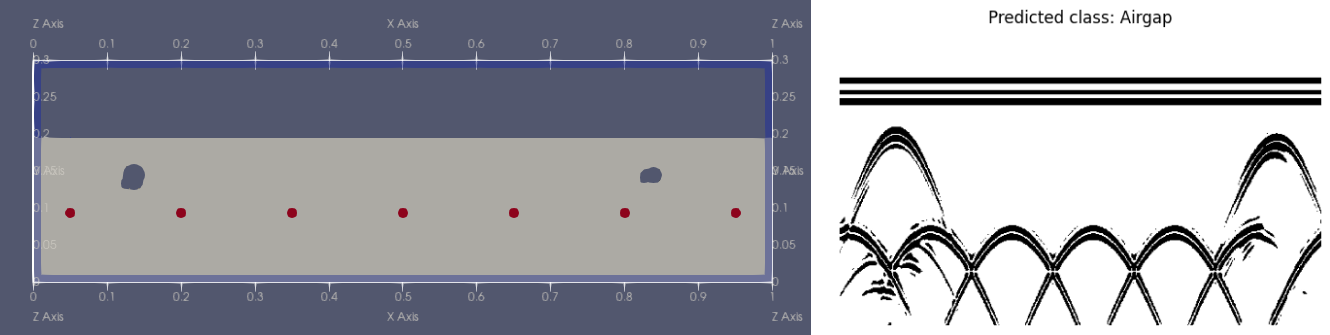
\includegraphics[scale=0.2]{gambar/bab4/Airgap 20007.png}
    \caption{Hasil Klasifikasi Percobaan Ketujuh 2}
\end{figure}

\begin{figure} [H] \centering
    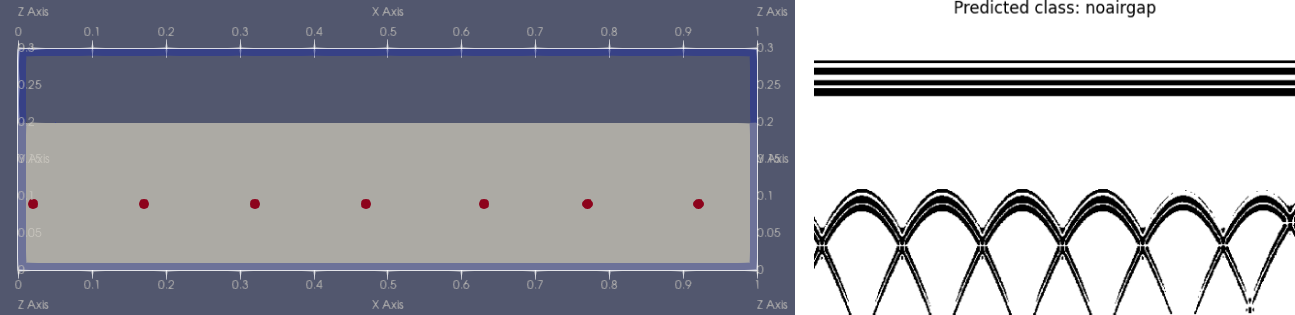
\includegraphics[scale=0.2]{gambar/bab4/Noarigap 19007.png}
    \caption{Hasil Klasifikasi Percobaan Ketujuh 3}
\end{figure}

\begin{figure} [H] \centering
    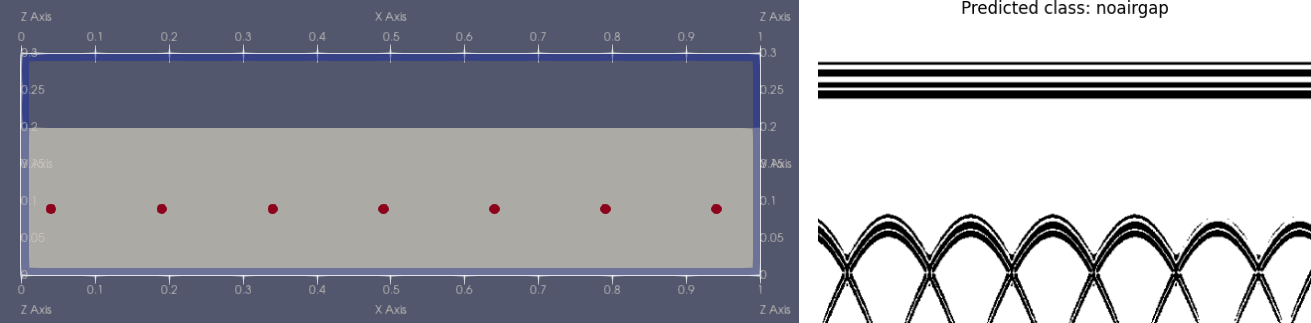
\includegraphics[scale=0.2]{gambar/bab4/Noairgap 20007.png}
    \caption{Hasil Klasifikasi Percobaan Ketujuh 4}
\end{figure}

Dari semua percobaan diatas, dapat diketahui bahwa hasil terbaik didapatkan pada percobaan kedua. Meskipun semua percobaan memiliki hasil klasifikasi yang baik, percobaan kedua memiliki hasil metrics yang lebih baik dibandingkan dengan percobaan lainnya. Hal tersebut dapat terlihat dari tabel \ref{tab:perbaningancnn} berikut.

\begin{table}[H]
    \centering
    \begin{tabular}{|c|c|c|c|c|c|c|}
        \hline
        \textbf{Percobaan ke} & \multicolumn{3}{c|}{\textbf{F1 Score}} & \multicolumn{3}{c|}{\textbf{Inference Time / step}}                                                \\ \cline{2-7}
                              & Training                               & Validation                                          & Testing    & Training & Validation & Testing \\ \hline
        1                     & 0.98926264                             & 1.0                                                 & 0.99750614 & 283ms    & 117ms      & 4s      \\ \hline
        2                     & 0.99714893                             & 1.0                                                 & 1.0        & 285ms    & 115ms      & 125ms   \\ \hline
        3                     & 0.99502486                             & 1.0                                                 & 1.0        & 301ms    & 114ms      & 1s      \\ \hline
        4                     & 0.961155                               & 0.98360646                                          & 0.9803921  & 281ms    & 162ms      & 2s      \\ \hline
        5                     & 0.92211217                             & 0.98684204                                          & 0.98360646 & 304ms    & 125ms      & 1s      \\ \hline
        6                     & 0.9985734                              & 1.0                                                 & 1.0        & 269ms    & 119ms      & 2s      \\ \hline
        7                     & 0.9985734                              & 1.0                                                 & 1.0        & 269ms    & 107ms      & 1s      \\ \hline
    \end{tabular}
    \caption{Tabel Perbandingan Hasil F1 Score dan Inference Time}
    \label{tab:perbaningancnn}
\end{table}

Berdasarkan tabel \ref{tab:perbaningancnn} diatas, dapat dilihat bahwa semua percobaan memiliki hasil F1 score dan inference time yang relatif sama. Akan tetapi, pada percobaan kedua, dihasilkan inference time yang paling cepat pada data testing dibandingkan dengan percobaan lainnya dengan selisih yang cukup besar. Oleh karena itu, percobaan kedua dipilih sebagai model terbaik untuk klasifikasi menggunakan CNN 2D.

\section{Pengujian Klasifikasi Roboflow}
\label{sec:PengujianRoboflow}
Proses klasifikasi menggunakan Roboflow hanya dilakukan satu kali dan hasil yang didapatkan akan dibandingkan dengan hasil klasifikasi menggunakan CNN 2-Dimensi. Hasil klasifikasi menggunakan Roboflow mendapatkan tingkat akurasi validasi sebesar 98.6\%. Selain itu, klasifikasi menggunakan juga menghasilkan grafik training loss dan valiation accuracy serta confusion matrix yang masing-masing dapat dilihat pada Gambar \ref{fig:roboflow} dan Gambar \ref{fig:confusionrobo}.

\begin{minipage}{\linewidth}
    \begin{figure} [H]
        \centering
        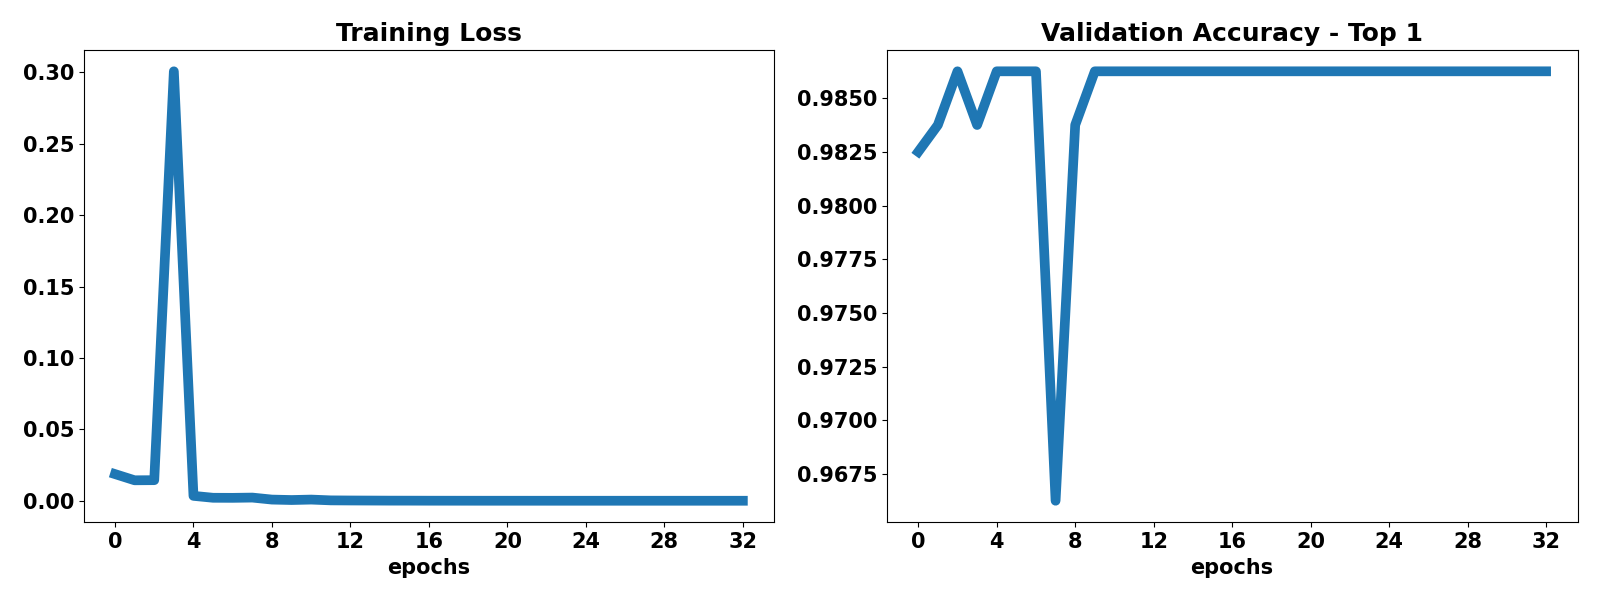
\includegraphics[scale=0.3]{gambar/bab4/roboflow.png}
        \caption{Hasil Training Loss dan Validation Accuracy Roboflow}
        \label{fig:roboflow}
    \end{figure}
\end{minipage}

\begin{minipage}{\linewidth}
    \begin{figure} [H]
        \centering
        \includegraphics[scale=1]{gambar/bab4/confusion.png}
        \caption{Confussion Matrix Roboflow}
        \label{fig:confusionrobo}
    \end{figure}
\end{minipage}

Dari hasil diatas, dapat didapatkan bahwa hasil klasifikasi menggunakan Roboflow memiliki tingkat akurasi yang cukup baik. Namun, hasil klasifikasi menggunakan Roboflow tidak dapat dijadikan sebagai acuan karena hanya dilakukan satu kali. Oleh karena itu, hasil klasifikasi menggunakan Roboflow akan dibandingkan dengan hasil klasifikasi menggunakan CNN 2-Dimensi serta akan diuji lagi melalui deteksi YOLOv9. Berikut ini merupakan hasil klasifikasi menggunakan Roboflow yang dapat dilihat pada gambar berikut:

\begin{figure} [H] \centering
    \includegraphics[scale=0.2]{gambar/bab4/robo1.png}
    \caption{Hasil Klasifikai Roboflow 1}
\end{figure}

\begin{figure} [H] \centering
    \includegraphics[scale=0.2]{gambar/bab4/robo2.png}
    \caption{Hasil Klasifikai Roboflow 2}
\end{figure}

\begin{figure} [H] \centering
    \includegraphics[scale=0.2]{gambar/bab4/robo3.png}
    \caption{Hasil Klasifikai Roboflow 3}
\end{figure}

\begin{figure} [H] \centering
    \includegraphics[scale=0.2]{gambar/bab4/robo4.png}
    \caption{Hasil Klasifikai Roboflow 4}
\end{figure}

\begin{figure} [H] \centering
    \includegraphics[scale=0.2]{gambar/bab4/robon.png}
    \caption{Hasil Klasifikai Roboflow 5}
\end{figure}

\section{Pengujian Deteksi YOLOv9}
\label{sec:PengujianYOLOv9}
Proses deteksi menggunakan YOLOv9 dilakukan sebanyak satu kali percobaan. Hasil klasifikasi menggunakan CNN 2-Dimensi dan Roboflow, nantinya akan dideteksi keberadaan rongga udaranya menggunakan YOLOv9 sehingga keberlangsungan pengujian deteksi menggunakan YOLOv9 sangat penting. Training YOLOv9 dilakukan dengan menggunakan dateset yang dilabeli melalui Roboflow. Dataset yang ada, dilakukan training dengan 10 epochs dan 8 batch. Dari hasil training, didapatkan hasil akurasi sebesar 0.979. Hasil metrics lainnya dapat dilihat pada gambar \ref{fig:metrics}. Selain itu, didapatkan pula hasil confusion matrix dari data training pada Gambar \ref{fig:conyolotrain}. Dari hasil tersebut, dapat dilihat bahwa hasil deteksi menggunakan YOLOv9 memiliki tingkat akurasi yang cukup tinggi.

\begin{figure} [H] \centering
    \includegraphics[scale=0.5]{gambar/bab4/metrics.png}
    \caption{Metrics YOLOv9}
    \label{fig:metrics}
\end{figure}

\begin{figure} [H] \centering
    \includegraphics[scale=0.1]{gambar/bab4/conyolotrain.png}
    \caption{Confussion Matrix YOLOv9}
    \label{fig:conyolotrain}
\end{figure}

Hasil confusion matrix diatas dapat terbentuk karena pada training YOLOv9 ini hanya digunakan satu kelas yakni kelas airgap atau rongga udara. Hal ini dilakukan karena pada penggunaan YOLOv9 ditunjukkan untuk mendeteksi satu objek saja yakni rongga udara pada sinyal B-Scan gprMax. Keakurasian YOLOv9 tersebut dapat dilihat dari hasil pengujian berikut dimana YOLOv9 mampu mendeteksi rongga udara pada sinyal B-Scan gprMax dengan baik. Berikut ini adalah contoh hasil deteksi menggunakan YOLOv9 yang dapat dilihat pada gambar berikut:

\begin{figure} [H] \centering
    \includegraphics[scale=0.2]{gambar/bab4/yolo1.png}
    \caption{Hasil Deteksi YOLOv9 1}
\end{figure}

\begin{figure} [H] \centering
    \includegraphics[scale=0.2]{gambar/bab4/yolo2.png}
    \caption{Hasil Deteksi YOLOv9 2}
\end{figure}

\begin{figure} [H] \centering
    \includegraphics[scale=0.2]{gambar/bab4/yolo3.png}
    \caption{Hasil Deteksi YOLOv9 3}
\end{figure}

\begin{figure} [H] \centering
    \includegraphics[scale=0.2]{gambar/bab4/yolo4.png}
    \caption{Hasil Deteksi YOLOv9 4}
\end{figure}